\section{Tecnologie utilizzate}

\subsection{Phonegap}\label{phonegap}

\subsubsection{Descrizione}
Phonegap è una distribuzione di Apache Cordova, ovvero una serie di API che permettono
di accedere a funzionalità di dispositivi mobile (come la fotocamera, sensori di posizione,
accelerometro) da codice Javascript. \\

Questo permette l'implementazione di applicazioni mobile cross platform a partire da 
tecnologie web, senza dover sviluppare codice nativo, tutto questo è gestito tramite il
servizio cloud \textit{Phonegap Build}\footnote{\texttt{ https://build.phonegap.com/}}. \\

\subsubsection{Vantaggi}

\paragraph{Prototipazione}
L'utilizzo di questo framework non ha influenzato tanto lo sviluppo dell'applicazione
per quanto è riguardato l'architettura della stessa o lo stile di codifica. La differenza
con altre esperienze di codifica mobile (SDK Android per il progetto del corso di Ingegneria
del Software) si è vista soprattutto nella rapidità di prototipazione permessa dal framework. \\
Phonegap permette di far partire l'applicazione sul browser o di scaricarla su di un
dispositivo mobile per poterla testare mano a mano che si aggiungono nuove componenti,
i cambiamenti infatti vengono riflessi automaticamente senza bisogno di risincronizzazione.

\paragraph{Adatto alla natura dell'applicazione}
\fiscoloMobile{} non richiede una complicata logica interna, né una base di dati complessa.
Uno sviluppo basato su un linguaggio nativo ad oggetti (ad esempio Java per Android) avrebbe
probabilmente complicato e appesantito il lavoro senza portare grandi vantaggi. \\

L'impressione che si ha è quella che questo framework possa rendere più agile e rapido
lo sviluppo di applicazioni (e che si adatti bene a uno sviluppo di tipo incrementale)
che abbiano soprattutto una natura \textit{front-end}.

\subsection{React}\label{react}

L'interfaccia utente di \fiscoloMobile{} è stata sviluppata sfruttando
questo framework. Seguono una breve descrizione dello stesso ed una valutazione
dei vantaggi riscontrati nel suo utilizzo.

\subsubsection{Descrizione}\label{descrizione-react}
La documentazione ufficiale di React lo definisce come un framework per applicazioni
che debbano gestire grandi quantità di dati che cambino nel tempo\footnote{\texttt{ http://facebook.github.io/react/docs/why-react.html}} e soprattutto
mostrare dinamicamente questi cambiamenti nella UI. \\

Una interfaccia utente è vista in React come un albero di \textbf{componenti}.
Una componente di React contiene tutte le informazioni necessarie a rappresentare
un elemento della vista in qualsiasi momento. \\

Ogni componente implementa una funzione \texttt{render} che crea una
\textit{rappresentazione} della stessa (i.e. una stringa di \gloss{markup}) e la inietta
poi nel documento (i.e. la pagina html). A un cambiamento nello stato della componente
segue una nuova renderizzazione, cioè la creazione di una nuova rappresentazione la quale
viene confrontata con quella precedente. Questo confronto permette di applicare
cambiamenti solo alle parti effettivamente modificate. Tutto questo processo è detto
di \textbf{riconciliazione} e permette di evitare la specifica di
\textit{\gloss{data-binding}} espliciti. \\

Altro aspetto importante è la possibilità di riutilizzo. In \fiscoloMobile{} 
ad esempio sono stati definiti dei componenti per ogni \textit{widget} grafico (e.g.
pulsanti, textbox, ecc.) i quali sono stati poi riutilizzati su tutte le pagine. \\

\subsubsection{Vantaggi}

\paragraph{Solo la View}\label{just-the-view}
L'utilizzo di React è stato trovato vantaggioso per lo sviluppo dell'applicazione.
\fiscoloMobile{} è infatti principalmente un'interfaccia che mostra e permette di
manipolare dati recuperati dalla controparte web. Questo suo aspetto ben si sposa
con la natura prettamente di \textit{view} del framework. \\

Sicuramente questa è una delle più grandi differenze da altri framework Javascript
come ad esempio Angular che si occupano di tutti gli aspetti del pattern \gloss{MVC}
(o \gloss{MVVM}, o \gloss{MVW}). \\

Da un lato questo è un vantaggio perché rende questa tecnologia leggera, semplice da
capire e rapida da imparare. Allo stesso tempo però ci si deve appoggiare ad altro
per avere indicazioni su come strutturare il substrato di questa \textit{view}. Per
questo si è fatto riferimento all'architettura Flux. \\

\paragraph{JSX}
Altro vantaggio riscontrato è stato la possibilità di utilizzare la sintassi JSX
la quale, unendo javascript e html, permette di definire le componenti in modo molto
intuitivo. Un esempio di tale sintassi è il seguente:

\begin{verbatim}
var Semaphore = React.createClass ({
  render : {
    return (
      <div>
        <span>
          {this.state.red ?
          Red :
          Green}
        </span>
      </div>	
    );
  }
});
\end{verbatim}

Questo permette di definire in modo molto semplice e rapido alcune proprietà dinamiche
delle componenti. Il suo vantaggio principale però è nel rendere chiara a colpo d'occhio
la struttura ad esempio di una pagina dell'applicazione la quale altro non è che una
componente "radice" di un albero di componenti e nodi html.

\subsubsection{Svantaggi}

\paragraph{Documentazione}
La documentazione presente sulla pagina ufficiale di React è stata sicuramente di aiuto
soprattutto per le fasi iniziali del progetto ma presenta alcuni aspetti potenzialmente
problematici:

\begin{itemize}
\item A prima vista è vagamente disorientante: sono presenti tre diverse guide di
\textit{quick start} (da quale iniziare?) e una serie di guide più approfondite che
non seguono però un ordine preciso. La documentazione non è insomma particolarmente
indirizzata ad utenti alle prime armi.
\item Non sono presenti particolari indicazioni su come strutturare applicazioni
a più pagine, l'assunzione che sembra permeare la maggior parte degli esempi e della
documentazione è che si debba sviluppare per una singola pagina.
\end{itemize}

\subsection{Flux}\label{flux}

Flux è un architettura per costruire applicazioni web lato client.

\subsubsection{Descrizione}

\begin{figure}[H]\label{imgFluxDataFlow}
	\centering
	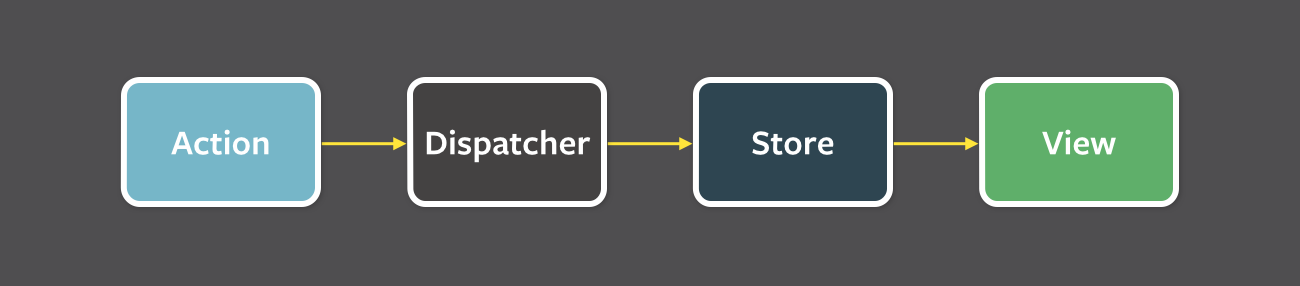
\includegraphics[width=1\columnwidth]{images/flux-data-flow.png}
	\caption{Il flusso dati di Flux}
\end{figure}

L'idea alla base dell'architettura è quella di un flusso di dati \textit{unidirezionale},
questo per rendere le applicazioni scalabili in dimensione senza crescita proporzionale
di complessità: il pericolo è quello di una serie di dipendenze tra le componenti e di reazioni
a catena ai cambiamenti che diventano difficilmente prevedibili in un sistema complesso. \\
Si cerca dunque di evitare questo lasciando che sia il \textit{model} stesso (che in questo caso
si può considerare come una versione aumentata del \textit{model} di MVC) a gestire i propri dati
e reagire ai cambiamenti, in modo del tutto trasparente all'esterno. \\

Un'applicazione Flux è composta dalle seguenti parti:

\begin{itemize}
\item \textbf{Store}: questi sono il modello dei dati (contengono la cosiddetta \textit{business
logic} dell'applicazione), tale modello non è però inerte, è compito degli Store infatti la
gestione dei dati e dei loro cambiamenti e la notifica di questi ultimi. Ogni Store si registra
su una componente detta \textit{Dispatcher} a determinate \textit{tipologie} di azioni (i.e.
input dall'esterno) e fornisce una funzione di callback che gestisce l'aggiornamento dei dati.
Espongono solo metodi \textit{getter}, i dati in input devono passare per il Dispatcher.
\item \textbf{View}: le viste di Flux si dividono in due sottocategorie:
	\begin{itemize}
	\item \textbf{Controller-View}: queste sono poste alla radice di un albero di componenti
	e hanno il compito di ascoltare i cambiamenti emessi in broadcast dagli Store e di aggiornare
	le viste subordinate quando necessario.
	\item \textbf{View semplici}: queste possono essere semplici componenti React che vengono
	aggiornate dalle Controller-View.
	\end{itemize}
\item \textbf{Dispatcher}: questa componente è unica per un'applicazione, offre metodi
che permettono agli Store di registrarsi per certe categorie di azioni. Inoltre offre la
possibilità di gestire le dipendenze tra gli Store e di strutturarli gerarchicamente.
\item \textbf{Action creators}: queste sono sostanzialmente librerie di funzionalità per le
diverse parti dell'applicazione. Non sono essenziali in quanto espongono metodi che
incapsulano chiamate al Dispatcher, aggiungono però molto valore in chiarezza e
comprensibilità del sistema in quanto offrono un'interfaccia che riassume tutti i cambiamenti
possibili all'interno dell'applicazione.
\end{itemize}

\paragraph{Nella pratica}
Questa architettura suggerisce una suddivisione del codice in package, per quanto riguarda
\fiscoloMobile{} la struttura (nelle sue parti relative a Flux) è la seguente:

\begin{itemize}
\item \texttt{actions}: contiene tutti gli action creators, suddivisi per pagina.
\item \texttt{components}: contiene tutte le pagine dell'applicazione, implementate tramite
componenti React.
	\begin{itemize}
	\item \texttt{common}: contiene tutte le componenti grafiche dell'applicazione.
	\end{itemize}
\item \texttt{constants}: definisce una serie di valori costanti, usati per distinguere
le diverse \textit{tipologie} di azioni.
\item \texttt{dispatcher}: contiene il Dispatcher dell'applicazione.
\item \texttt{stores}: contiene uno Store per ogni pagina, più uno di utilità generale e uno
per la navigazione.
\end{itemize}

\paragraph{Un esempio}
Per capire le relazioni tra le diverse componenti può essere utile vedere un esempio. \\

Si consideri il text field utilizzato nella schermata di login di \fiscoloMobile{},
come spiegato in sezione \ref{password}, è possibile mascherare o meno il testo
inserito tramite un bottone.
Le componenti in gioco sono dunque:

\begin{itemize}
\item \texttt{LoginPage}: questa è la \textit{Controller-View} che gestisce l'intera
pagina di login, al caricamento si registra come ascoltatrice dei cambiamenti emessi
da \texttt{LoginStore} e fornisce una funzione di callback \texttt{onChange}.
\item \texttt{FiscoloTextInput}: questa è la \textit{View} relativa al campo password
della pagina di login, il suo stato è mantenuto da \texttt{LoginPage}.
\item \texttt{FiscoloIconButton}: la \textit{View} relativa al bottone da cliccare per
aggiungere o togliere la mascheratura alla password.
\item \texttt{LoginActions}: qui sono riassunti tutti i possibili cambiamenti causati
da azioni esterne all'applicazione, in particolare vi è un metodo \texttt{switchPasswordType}
che permette di aggiungere o togliere la mascheratura.
\item \texttt{LoginStore}: qui è contenuto lo stato della pagina e qui avvengono effettivamente
i cambiamenti suscitati dalle azioni.
\end{itemize}

Un click sul bottone causa questa catena di eventi:

\begin{enumerate}
\item Viene invocata la funzione \texttt{switchPasswordType} di \texttt{LoginPage} che
chiama a sua volta la omonima di \texttt{LoginActions}.
\item Tale invocazione fa sì che il \textit{Dispatcher} trasmetta in broadcast un'azione con
tipologia \texttt{Constants.LOGIN\_SWITCH\_PASSWORD\_TYPE}.
\item L'azione viene ascoltata da \texttt{LoginStore} che invoca dunque la sua funzione
di callback che consiste di uno \textit{switch} che smista le azioni (in base alla tipologia)
chiamando diverse funzioni. La tipologia dell'azione causa quindi l'invocazione della
funzione \texttt{switchPasswordType} di \texttt{LoginStore}.
\item Tale funzione modifica i dati all'interno dello \textit{Store}, in particolare cambia un
campo dati contenente la tipologia della stringa e un campo dati contenente il nome
dell'icona del bottone.
\item Dopo questi cambiamenti la funzione emette in broadcast un evento di \textit{cambiamento}.
\item \texttt{LoginPage}, essendosi registrata ai cambiamenti emessi da \texttt{LoginStore},
invoca la sua funzione di callback \texttt{onChange} che, usando i metodi getter offerti dallo
\textit{Store}, recupera tutti i dati necessari ad aggiornare lo stato. L'invocazione di questo metodo
fa partire inoltre un nuovo ciclo di rendering e la vista viene così aggiornata (la password
sarà mascherata o meno, l'icona mostrerà un occhio aperto o chiuso).
\end{enumerate}


\subsubsection{Vantaggi}

\paragraph{Integrazione con React}
React e Flux sono due tecnologie che si completano e complementano a vicenda. Da un lato
Flux sopperisce alla mancanza di indicazioni su come strutturare il substrato della vista
di un'applicazione da parte di React (cfr. \ref{just-the-view}). Dall'altro lato React,
nascondendo i dettagli su come vengano effettivamente aggiornati gli elementi della pagina
tramite il metodo \texttt{render} (cfr. \ref{descrizione-react}), rende intuibile il flusso
di dati di Flux.

\paragraph{Scalabilità}
L'unidireazionalità del flusso di dati all'interno delle applicazioni Flux impedisce
l'esplosione della complessità al crescere di un sistema: non sono possibili scambi di
dati arbitrari tra View e Controller, ogni View è in ascolto su un certo numero di Store,
ogni Store ha come unico punto di accesso delle azioni che passano attraverso il Dispatcher. \\

Una volta compresa questa struttura, l'aggiunta di nuove pagine e funzionalità
ha sempre seguito lo stesso schema.

\paragraph{Debugging}
Un movimento di dati prevedibile ha permesso operazioni di debugging più efficienti.

\subsubsection{Svantaggi}

\paragraph{Documentazione}
Sul sito ufficiale di Flux sono offerte alcune guide di \textit{quick start} e poca
altra documentazione. Queste permettono di capire abbastanza bene l'idea alla base
del'architettura, la relazione tra le diverse componenti ecc. Tuttavia entrambe le
applicazioni usate come esempio sono a singola pagina e non vengono fornite indicazioni
su come gestire un sistema di navigazione. \\
Questo ha causato qualche problema nelle fasi iniziali del progetto in quanto non
mi era molto chiaro come gestire il passaggio tra le diverse pagine dell'applicazione. \\
Il problema è stato infine risolto costruendo un apposito \textit{Store} di navigazione
che si mette in ascolto di una categoria di azioni \texttt{Constants.NAV\_*} e si occupa
della renderizzazione delle nuove pagine. \\
Tale soluzione è risultata funzionale per l'applicazione ma non è chiaro se sia una modalità
ideale per l'architettura, o se ci possano essere soluzioni migliori.

\subsection{Material Ui}\label{material-ui}

Questa libreria è stata utilizzata per implementare un'interfaccia utente il più
possibile conforme ai principi di material design.

\subsubsection{Descrizione}
Le componenti grafiche (come bottoni, textbox, barre di navigazione ecc.) vengono
fornite come normali componenti React con attributi, metodi ed eventi associati.

\subsubsection{Vantaggi}

\paragraph{Rispetto dei principi di material}
Le componenti rispecchiano in larga
misura quanto stabilito nella documentazione di material design e sono facilmente 
utilizzabili in ambiente React.

\subsubsection{Svantaggi}\label{svantaggi-material-ui}

\paragraph{Scarsa documentazione}
La documentazione di Material Ui consiste soprattutto
di brevi snippet di codice mostrati come esempio, mancano riferimenti più approfonditi ed
esempi completi. In alcune occasioni è stato necessario studiare il sorgente\footnote{\texttt{ https://github.com/callemall/material-ui}} per capire il
funzionamento di alcune componenti.

\paragraph{Poca libertà di azione}
La personalizzazione delle diverse componenti non è
semplice. In certi casi vengono offerti degli attributi che permettono di sovrascriverne
lo stile con css personale, in altri casi è stato necessario scrivere codice css piuttosto
complicato per raggiungere i nodi rilevanti.

\paragraph{Problemi con alcuni widget}
Si è riscontrato un problema non documentato
per il widget dei menù a tendina: la selezione di un nuovo elemento causava un errore
segnalato dall'inspector di Chrome con il messaggio \textit{console.assert
is not a function}. Tale funzione viene infatti invocata dal codice della componente
\texttt{DropDownMenu} di Material Ui. Non è stata trovata documentazione di alcun tipo
riguardo questo errore e il problema è stato risolto ridefinendo il metodo
\texttt{console.assert} come un \gloss{NOOP}.

\paragraph{Mancanza di supporto alle transizioni}
Non sono stati trovati riferimenti
o documentazione a riguardo delle transizioni e in generale di animazioni che andassero
oltre un semplice \textit{touch ripple}. Questi aspetti sono però molto importanti per
material design (cfr. \ref{material-animation}).

\subsection{Chart.js}

\subsubsection{Descrizione}
Era previsto l'utilizzo di questa libreria per mostrare i diversi grafici delle pagine
di reportistica di \fiscoloMobile{}. Tali pagine non sono però state sviluppate (cfr.
sezione \ref{esiti}).

\subsubsection{Vantaggi}

\paragraph{Ottima integrazione con React}
Nonostante il mancato utilizzo nell'applicazione finale la libreria è stata comunque
testata in una fase iniziale, è stato utilizzato il modulo \texttt{react-chartjs} per
React e sono stati fatti alcuni test di integrazione. Tali test hanno dato buoni
risultati ai primi tentativi, l'impressione ricavata è stata dunque molto buona.

\begin{figure}[H]\label{imgChartJS}
	\centering
	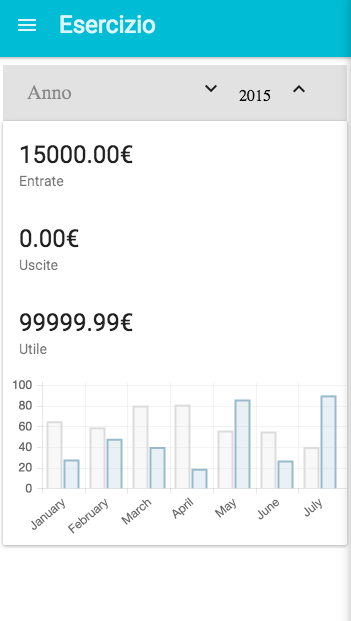
\includegraphics[width=.4\columnwidth]{images/chartjs.png}
	\caption{Screenshot da una schermata statica prodotta come test di integrazione}
\end{figure}

\begin{table} [H] \centering
\begin{tabularx}{\textwidth}{|c|X|}
\hline
\textbf{Phonegap} & \\ \hline
\textit{Vantaggi}
& Rapidità di prototipazione \\ \hline
& Adatto per applicazioni semplici che fungano principalmente da interfacce per mostrare dati \\ \hline \hline
\textbf{React} & \\ \hline
\textit{Vantaggi}
& Leggerezza del framework (concentrato sulla parte di \textit{View}) adatta alla natura dell'applicazione da implementare \\ \hline
& Sintassi JSX intuitiva e potente, lasciando comunque la libertà di utilizzare Javascript puro \\ \hline
\textit{Svantaggi}
& Documentazione vagamente disorientante e non troppo chiara su alcuni aspetti \\ \hline \hline
\textbf{Flux} & \\ \hline
\textit{Vantaggi}
& Perfetta integrazione con React \\ \hline
& Comprensibilità e scalabilità una volta appresi meccanismi e il flusso dati \\ \hline
& Debugging semplificato dal flusso dati unidirezionale \\ \hline 
\textit{Svantaggi}
& Documentazione scarsa e con lacune su aspetti importanti del progetto (navigazione) \\ \hline
\hline
\textbf{Material Ui} & \\ \hline
\textit{Vantaggi}
& Buona implementazione degli aspetti grafici (forma, spazi, ecc.) di material design \\ \hline
& Buona integrazione con React \\ \hline
\textit{Svantaggi}
& Scarsa documentazione \\ \hline
& Poca libertà d'azione, di customizzazione dei componenti \\ \hline
& Mancanza di supporto e documentazione riguardo le transizioni \\ \hline \hline
\textbf{Chart.js} & \\ \hline
\textit{Vantaggi}
& Ottima integrazione con React tramite il modulo \texttt{react-chartjs} \\ \hline
\end{tabularx}
\caption{Riassunto della valutazione delle tecnologie utilizzate}
\end{table}